\documentclass[11pt]{article}
\usepackage[a4paper,margin=1.8cm]{geometry}
\usepackage{amsmath, amssymb, amsthm}  % Essential math packages
\usepackage{graphicx}                   % For figures
\usepackage{hyperref}                   % Clickable links
\usepackage{parskip} % cleaner spacing
\usepackage{enumitem}
\usepackage{mdframed}
\usepackage{titlesec}
\newcommand{\sectionbreak}{\clearpage}

\usepackage{listings}
\usepackage{xcolor}



\lstset{
  language=Python,
  basicstyle=\ttfamily\small,
  keywordstyle=\color{blue},
  stringstyle=\color{red},
  commentstyle=\color{green!50!black},
  showstringspaces=false,
  breaklines=true
}

% Define a solution environment with a box
\newenvironment{solbox}
  {\begin{mdframed}[linewidth=1pt,linecolor=black,roundcorner=5pt]
   \noindent\textbf{Ans: }\enspace}
  {\end{mdframed}}


\title{Assigment 1 \\ MAT3110 - Introduction to numerical analysis}
\author{Oliver Ekeberg}
\date{\today}

\begin{document}
\maketitle


\tableofcontents

\section{Exercise 1}

Use the QR factorization of A and apply back substitution to R1 to
find x. You will need to write your own routine for back substitution
but you can use the matlab function
[Q,R] = qr(A);
to find Q and R.


\begin{solbox}

    \subsection{Back-substitution implementation}
    

    I used the built in function for Q and R calculations from numpy. I implemented the following function for back substitution:

    \begin{lstlisting}[language=Python]
        def back_subst(A: np.ndarray, b: np.ndarray):
            n = b.shape[0]
            if A.shape[0] != A.shape[1]:
                raise ValueError("Input must be square, douche...")
            x = np.zeros(n)
            x[n-1] = b[n-1] / A[n-1, n-1]

            for i in range(n-2, -1, -1):
                x[i] =  (b[i] - A[i, i+1:] @ x[i+1:]) / A[i,i]
            return x
    \end{lstlisting}
    \begin{itemize}
        \item The code takes input square a upper triangle matrix, and an arbitrary vector b that takes the same shape as the rows and columns of A
        \item Then I loop backwards from the lower diagonal and up. I have equations of the following form
        \[
            \sum_{ j=n }^{ n-j } \sum_{ i=j+1 }^{ j=n } a_{ji} x_j = b_j 
        \]
        And we can solve this by taking the dot product of th
        
    
    \end{itemize}
    

    \subsection{QR plots for both datasets, only m=3}
    
    \subsubsection{QR plot for dataset 1 m=3}
    
    This produced the following plot for data set 1:

    \begin{center}
    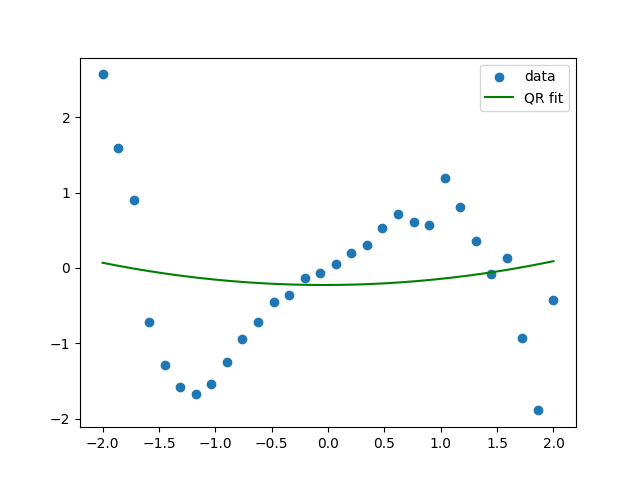
\includegraphics[width=0.75\linewidth]{../Figures/M3QR_plot_dataset1.png}
    \end{center}

    \subsubsection{QR plot for dataset 2 m=3}
    
    And the following plot for dataset 2:
    \begin{center}
    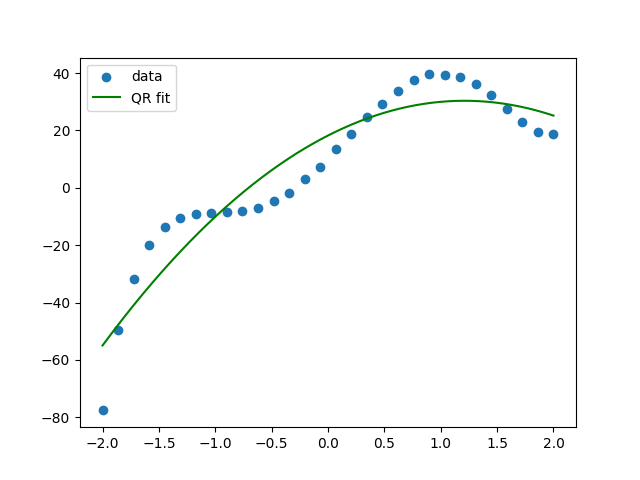
\includegraphics[width=0.75\linewidth]{../Figures/M3QR_plot_dataset2.png}
    \end{center}


    \subsection{QR plot for both datasets, only m=8}
    

    \subsubsection{QR plot for dataset1 m=8}
    And here is the plot for the QR coefficients for dataset 1, $ m=8 $ 

    \begin{center}
    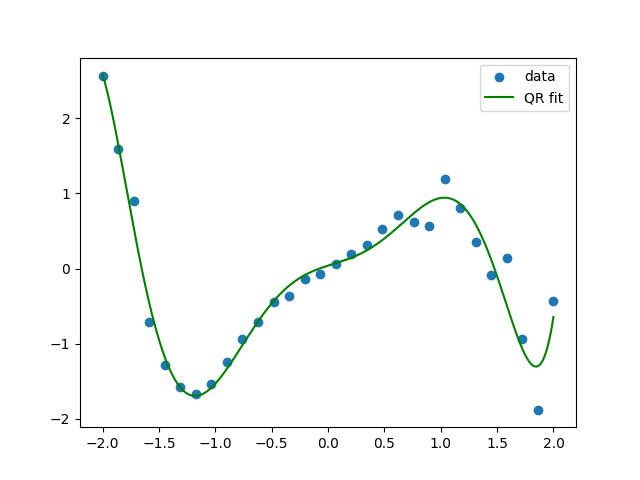
\includegraphics[width=0.75\linewidth]{../Figures/M8QR_plot_dataset1.png}
    \end{center}
    

    \subsubsection{QR plot for dataset2 m=8}
    And here is the plot for the QR coefficients for dataset 2, $ m=8 $ 
    
    
    \begin{center}
    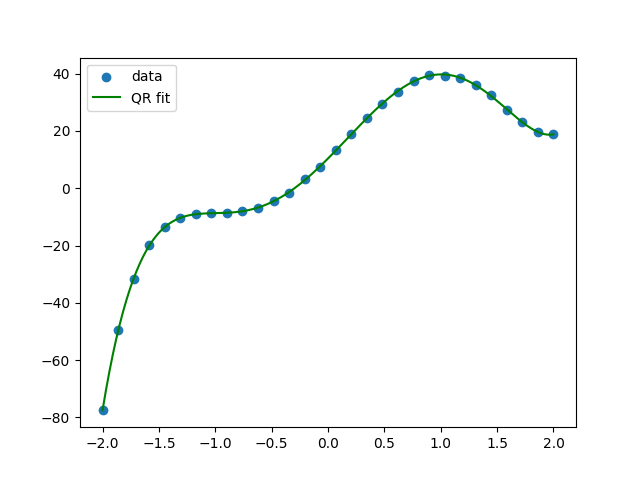
\includegraphics[width=0.75\linewidth]{../Figures/M8QR_plot_dataset2.png}
    \end{center}

\end{solbox}


\section{Exercise 2}

The $m x m$ matrix $B = A^T A$ is symmetric and positive definite. Solve the normal equations using the Cholesky factorization $RR^T$ of $B$. To do
this you also need to implement forward substitution and the Cholesky
algorithm explained in Lecture 3.


\begin{solbox}
    \subsection{Cholesky implementation}

    Here is my Cholesky implementation.



    \begin{lstlisting}[language=Python]
        def cholesky(A):
            A = A.copy().astype(float)
            n = A.shape[0]
            L = np.zeros((n,n))
            D = np.zeros((n,n))
            for i in range(n):
                lk = A[:,i] / A[i,i]
                L[:,i] = lk
                D[i,i] = A[i,i] 
                A = A - D[i,i] * np.outer(lk, lk)
            return L, D
    \end{lstlisting}

    Here is the figure for the Cholesky interpolation for dataset 1

    \subsection{Cholesky plot for both datasets, only  m=3}


    \subsubsection{Cholesky plot for dataset 1 m=3}
    

    plott 1 for cholesky
    \begin{center}
    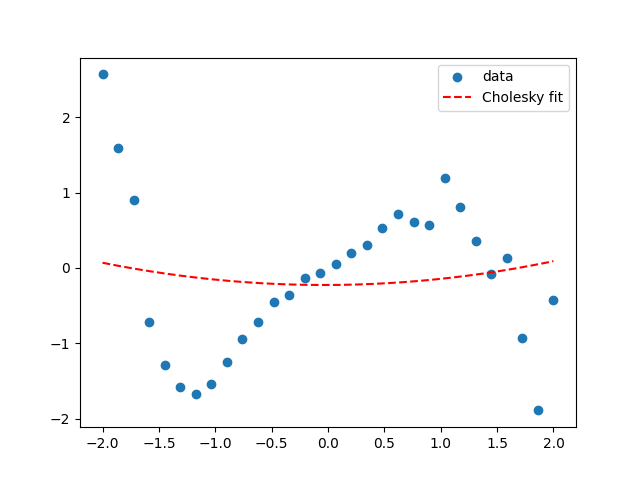
\includegraphics[width=0.75\linewidth]{../Figures/M3Chol_plot_dataset1.png}
    \end{center}

    \subsubsection{Cholesky plot for dataset 2 m=3}

    here is the second plot 
    \begin{center}
    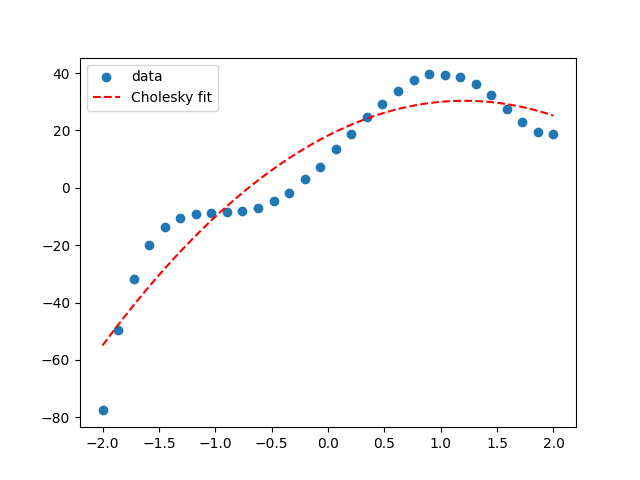
\includegraphics[width=0.75\linewidth]{../Figures/M3Chol_plot_dataset2.png}
    \end{center}

    \subsection{Plots for both datasets, only m=8}

    Both plots for Cholesky factorization, m=8
    
    \subsubsection{Cholesky plot for dataset1 m=8}

    \begin{center}
    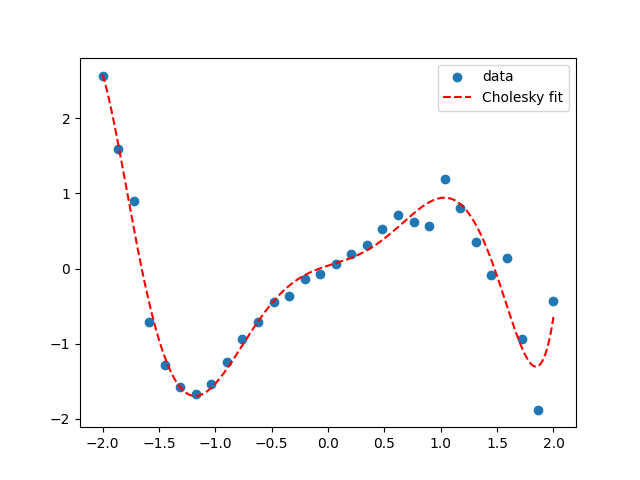
\includegraphics[width=0.75\linewidth]{../Figures/M8Chol_plot_dataset1.png}
    \end{center}


    \subsubsection{Cholesky plot for dataset2 m=8}

    \begin{center}
    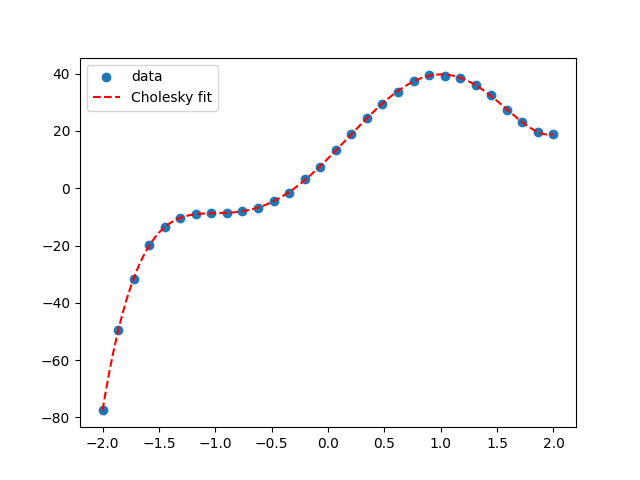
\includegraphics[width=0.75\linewidth]{../Figures/M8Chol_plot_dataset2.png}
    \end{center}



    

\end{solbox}


\section{Exercise 3}

Here I will discuss the differences

\begin{solbox}
    In a linear system, we have several possible outcomes for our solutions to $ Ax=b$
    
    \begin{itemize}
        \item One unique solution
        \item infinite solutions
        \item no solutions
    \end{itemize}

    Very often, we might not have any solution. We can still find the best approximation of this soltion, by finding the x that minimizes the distance between $ Ax $ and $ b $. In other words, finding where the projection onto b is the smallest. 

    \[
         \|b-A \hat{x} \|_2 = min_x \|b - Ax \|_2
    \] 

    The 2 indicates which norm. We can find the condition number $ K(A) = \frac{\sigma_{max}} {\sigma_{min}} $ 
    

    \subsection{Table of Condition number for $ A $ , given different m}
    
    Here is a brief overview over the condition number of A, given m



    \begin{center}
    \begin{tabular}{||c c c c||} 
    \hline
    K(A) & m \\ [0.5ex] 
    \hline
    $ 3.35669965 \approx 3.36  $  & 3 \\ 
    \hline
    $ 508.8654270541882 \approx 508.87 $  & 8 \\
    \hline
    $ 773972758.7055001 \approx 774 * 10^{6} $  & 20 \\ 
    \hline
    \end{tabular}
    \end{center}


    We see here that using the Vanderbild matrix for the QR factorization, is very ill-conditioned. And we will have to restrict ourselves to small m, or expect large rounding errors. 

    \subsection{Table of Condition number for $ A^TA $ , given different m}

    This is only for the QR factorization, for the Cholesky factorization, we computed $A^T A$

    \begin{center}
    \begin{tabular}{||c c c c||} 
    \hline
    $ A^TA $  & m \\ [0.5ex] 
    \hline
    $ 11.267432570084102 \approx 11.27  $  & 3 \\ 
    \hline
    $ 258944.02285017748 \approx 2.6 * 10^4 $  & 8 \\
    \hline
    $ 6.067836823000123e+17 $  & 20 \\ 
    \hline
    \end{tabular}
    \end{center}

    So for the normal equations, we are extremely ill-conditioned for large m. From this, we prefer the QR method for solving   

    \[
         min_x \| AX - b\|_2
    \] 

    But this comes at a cost of computational complexity. Instead of orthogonalizing columns of A, as QR does, Cholesky only builds a smaller m x m matrix $ A^TA $ and factorize it. It approximately halves arithmetic, but at the expense of computational cost. So by increasing the number of polynomials we use to approximate the function (m), we will have diminishing returns by picking the Cholesky normal equations approach. 

\end{solbox}


\section{Appendix: Code }


\begin{lstlisting}[language=Python]
    import numpy as np
    import matplotlib.pyplot as plt

    np.set_printoptions(linewidth=np.inf)

    n = 30
    m=20
    start = -2
    stop = 2
    x = np.linspace(start, stop, n)
    eps = 1
    np.random.seed(1)
    r = np.random.rand(n) * eps
    y = x * np.cos(r + 0.5 * x**3) + np.sin(0.5 * x**3)
    y2 = 4 * x**5 - 5 * x**4 - 20 * x**3 + 10 * x**2 + 40 * x + 10 + r

    v = np.vander(x, N = m, increasing = True)
    singular_values_V = np.linalg.svd(v.T @ v)[1]
    singular_values_VTV = np.linalg.svd(v.T @ v)[1]
    KA_V = singular_values_V[0] / singular_values_V[-1]
    KA_VTV = singular_values_VTV[0] / singular_values_VTV[-1]


    print(f"Singular values for\n" \
    "--------------------------------------------\n" \
    "V: {KA_V}\n" \
    "VTV: {KA_VTV}")

    def back_subst(A: np.ndarray, b: np.ndarray):
        n = b.shape[0]
        if A.shape[0] != A.shape[1]:
            raise ValueError("Input must be square, douche...")
        x = np.zeros(n)
        x[n-1] = b[n-1] / A[n-1, n-1]

        for i in range(n-2, -1, -1):
            x[i] =  (b[i] - A[i, i+1:] @ x[i+1:]) / A[i,i]
        return x


    def cholesky(A):
        A = A.copy().astype(float)
        n = A.shape[0]
        L = np.zeros((n,n))
        D = np.zeros((n,n))
        for i in range(n):
            lk = A[:,i] / A[i,i]
            L[:,i] = lk
            D[i,i] = A[i,i] 
            A = A - D[i,i] * np.outer(lk, lk)
        return L, D


    def cholesky2(B):
        n = B.shape[0]
        L = np.zeros_like(B)
        for i in range(n):
            L[i,i] = np.sqrt(B[i,i] - np.sum(L[i,:i]**2))
            for j in range(i+1, n):
                L[j,i] = (B[j,i] - np.sum(L[j,:i]*L[i,:i])) / L[i,i]
        return L

    def forward_subst(A: np.ndarray, b: np.ndarray):
        '''A: nxn matrix, b: nx1 matrix'''
        n = A.shape[0]
        x = np.zeros(n)
        x[0] = b[0] / A[0,0]
        for i in range(1, n):
            x[i] = (b[i] - np.dot(A[i, :i], x[:i])) / A[i,i]
        return x

    def solve_cholesky(V, y):
        B = V.T @ V
        L = np.linalg.cholesky(B)   
        b = V.T @ y
        z = forward_subst(L, b)
        c = back_subst(L.T, z)
        return c


    def fit_and_plot(dataset, m, x):
        V = np.vander(x, N=m, increasing=True)

        # --- QR method
        Q, R = np.linalg.qr(V)
        coefs_qr = back_subst(R, Q.T @ dataset)

        # --- Normal equations with Cholesky
        B = V.T @ V
        L = np.linalg.cholesky(B)
        b = V.T @ dataset
        z = forward_subst(L, b)
        coefs_chol = back_subst(L.T, z)

        # poly1d wants descending order
        p_qr = np.poly1d(coefs_qr[::-1])
        p_chol = np.poly1d(coefs_chol[::-1])

        xx = np.linspace(x.min(), x.max(), 400)
        plt.scatter(x, dataset, label="data")
        plt.plot(xx, p_qr(xx), 'g-', label="QR fit")
        #plt.plot(xx, p_chol(xx), 'r--', label="Cholesky fit")
        plt.legend()
        plt.show()

    fit_and_plot(dataset = y, m=20, x = x)



\end{lstlisting}




\end{document}
